% *********************************************************************
% © 2021 Jeremy Sylvestre
%
% Permission is granted to copy, distribute and/or modify this document
% under the terms of the GNU Free Documentation License, Version 1.3 or
% any later version published by the Free Software Foundation; with no
% Invariant Sections, no Front-Cover Texts, and no Back-Cover Texts. A
% copy of the license is included in the appendix entitled “GNU Free
% Documentation License” that appears in the output document of this
% PreTeXt source code. All trademarks™ are the registered® marks of
% their respective owners.
%
% *********************************************************************

\newcommand*{\xmin}{-1}
\newcommand*{\xmax}{11}
\newcommand*{\ymin}{-0.5}
\newcommand*{\ymax}{1}

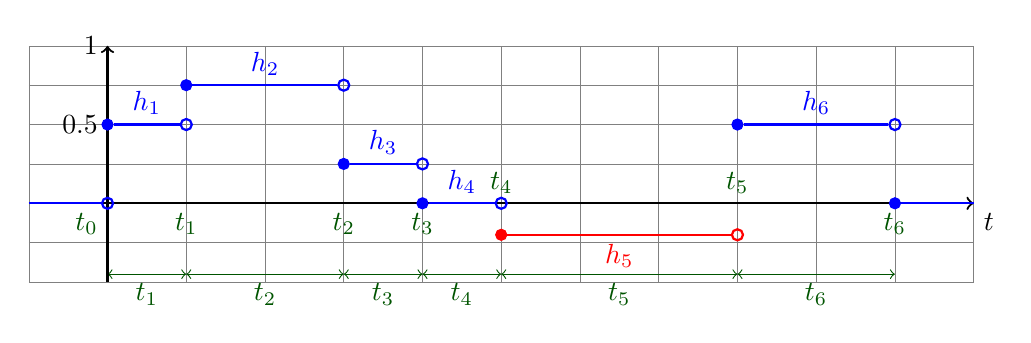
\begin{tikzpicture}
[
	closedpt/.style={circle,draw,fill,inner sep=0pt,minimum size=4pt},
	openpt/.style={circle,draw,inner sep=0pt,minimum size=4pt},
	yscale=2
]

	% grid
	\foreach \x in {-1,0,1,...,11} {
		\draw[very thin,gray] (\x,\ymin) -- (\x,\ymax);
	}
	\foreach \y in {-0.5,-0.25,0,0.25,...,1} {
		\draw[very thin,gray] (\xmin,\y) -- (\xmax,\y);
	}

	% label grid
	\node[below left,green!33!black] at (0,0) {$t_0$};
	\node[below,green!33!black] at (1,0) {$t_1$};
	\node[below,green!33!black] at (3,0) {$t_2$};
	\node[below,green!33!black] at (4,0) {$t_3$};
	\node[above,green!33!black] at (5,0) {$t_4$};
	\node[above,green!33!black] at (8,0) {$t_5$};
	\node[below,green!33!black] at (10,0) {$t_6$};

	% interval widths
	\draw[green!33!black,<->] (0,-0.45)
	  -- node[below] {$\change{t_1}$}
	  (1,-0.45)
	;
	\draw[green!33!black,<->] (1,-0.45)
	  -- node[below] {$\change{t_2}$}
	  (3,-0.45)
	;
	\draw[green!33!black,<->] (3,-0.45)
	  -- node[below] {$\change{t_3}$}
	  (4,-0.45)
	;
	\draw[green!33!black,<->] (4,-0.45)
	  -- node[below] {$\change{t_4}$}
	  (5,-0.45)
	;
	\draw[green!33!black,<->] (5,-0.45)
	  -- node[below] {$\change{t_5}$}
	  (8,-0.45)
	;
	\draw[green!33!black,<->] (8,-0.45)
	  -- node[below] {$\change{t_6}$}
	  (10,-0.45)
	;

	\foreach \y in {0.5,1} {
		\node[left] at (0,\y) {$\y$};
	}

	% axes
	\draw[->,thick] (\xmin,0) -- (\xmax,0) node[below right] {$t$};
	\draw[->,thick] (0,\ymin) -- (0,\ymax);

	% off
	\node[blue,thick,openpt] at (0,0) (stop) {};
	\draw[blue,thick] (\xmin,0) -- (stop);

	% medium
	\node[blue,closedpt] at (0,0.5) (mstart) {};
	\node[blue,thick,openpt] at (1,0.5) (mstop) {};
	\draw[blue,thick] (mstart) -- (mstop);

	% high
	\node[blue,closedpt] at (1,0.75) (hstart) {};
	\node[blue,thick,openpt] at (3,0.75) (hstop) {};
	\draw[blue,thick] (hstart) -- (hstop);

	% low
	\node[blue,closedpt] at (3,0.25) (lstart) {};
	\node[blue,thick,openpt] at (4,0.25) (lstop) {};
	\draw[blue,thick] (lstart) -- (lstop);

	% off
	\node[blue,closedpt] at (4,0) (start) {};
	\node[blue,thick,openpt] at (5,0) (stop) {};
	\draw[blue,thick] (start) -- (stop);

	% leaking
	\node[red,closedpt] at (5,-0.2) (start) {};
	\node[red,thick,openpt] at (8,-0.2) (stop) {};
	\draw[red,thick] (start) -- (stop);

	% medium
	\node[blue,closedpt] at (8,0.5) (start) {};
	\node[blue,thick,openpt] at (10,0.5) (stop) {};
	\draw[blue,thick] (start) -- (stop);

	% off
	\node[blue,closedpt] at (10,0) (start) {};
	\draw[blue,thick] (start) -- (\xmax,0);

	% label heights
	\node[above,blue] at (0.5,0.5) {$h_1$};
	\node[above,blue] at (2,0.75) {$h_2$};
	\node[above,blue] at (3.5,0.25) {$h_3$};
	\node[above,blue] at (4.5,0) {$h_4$};
	\node[below,red] at (6.5,-0.2) {$h_5$};
	\node[above,blue] at (9,0.5) {$h_6$};

\end{tikzpicture}
